\subsection{Using kernels}

Let's look again at the \textbf{Wolfe dual Lagrangian problem}, but this time applied to the dimension-lifting trick from before.
\begin{align*}\begin{aligned}
  &\text{For } \cv{w}=\sum_{i=1}^m \alpha_i y_i \cv{x}_i \text{ and } \alpha_i\geq0, i=1,\dots,m \sidenote{Wolfe dual Lagrangian problem with kernel}\\
  & \begin{array}{rl}
      \max_\alpha & \sum_{i=1}^m \alpha_i - \frac{1}{2} \sum_{i=1}^m \sum_{j=1}^m \alpha_i \alpha_j y_i y_j \underbrace{\color{burntorange}K(\cv{x}_i,\cv{x}_j)}_{=\phi(\cv{x}_i)\cdot\phi(\cv{x}_j)}\\
      \text{subject to } & \sum_{i=1}^m \alpha_i y_i = 0
  \end{array}
\end{aligned}\end{align*}
\begin{itemize}
  \item Once again, we have $\phi\in\mathbb{R}^n\rightarrow\mathbb{R}^q$ with $q>n$
  \item $K$ is our \textbf{kernel function}\sidenote{Kernel function}
  \begin{itemize}
    \item It efficiently computes $\phi(\cv{x}_i)\cdot\phi(\cv{x}_j)$
    \item S.t., the actual mapping mappings $\phi(\cv{x}_i)$ and $\phi(\cv{x}_j)$ as well as their dot product don't need to be computed
  \end{itemize}
\end{itemize}

\begin{note}
Consider the kernel function for our previous example \ref{fig:5_not_linear_separable}.
\begin{align*}
  \phi(x_1, x_2) &= \left(x_1^2, \sqrt{2}x_1x_2, x_2^2\right) \\
  \implies \phi(x_{i/j,1}, x_{i/j2}) &= \left(x_{i/j,1}^2, \sqrt{2}x_{i/j,1}x_{i/j,2}, x_{i/j,2}^2\right)\\
  \implies K(\cv{x}_i, \cv{x}_j) = \phi(\cv{x}_i)\cdot\phi(\cv{x}_j) &= \underbrace{x_{i,1}^2x_{j,1}^2}_{(x_{i,1}x_{j,1})^2} + \underbrace{2x_{i,1}x_{i,2}x_{j,1}x_{j,2}}_{2(x_{i,1}x_{j,1})(x_{i,2}x_{j,2})} + \underbrace{x_{i,2}^2x_{j,2}^2}_{(x_{i,2}x_{j,2})^2}\\
  &= (x_{i,1}x_{j,1} + x_{i,2}x_{j,2})^2
\end{align*}
\begin{itemize}
  \item So, for calculating $\phi(\cv{x}_i)\cdot\phi(\cv{x}_j)$, we need 10 multiplication-operations and 2 addition-operations,
  \item Whereas for calculating $K(\cv{x}_i, \cv{x}_j)$, we need 3 multiplication-operations and 1 addition-operation.
\end{itemize}
\end{note}

In the following, we'll see some kernel functions:
\begin{itemize}
  \item We can use \textbf{polynomial kernels} with parameters $c$ (constant) and $d$ (degree, remember the danger of overfitting with increasing degree).
  \begin{align*}
    K(\cv{x}_i, \cv{x}_j) &= \underbrace{\phi(\cv{x}_i) \cdot \phi(\cv{x}_j)}_{\phi \text{ may have a variable (large) number of dimensions}} = (\cv{x}_i\cdot\cv{x}_j + c)^d
  \end{align*}
  \begin{figure*}[ht]
    \centering
    \begin{subfigure}{0.2\textwidth}
      \centering
      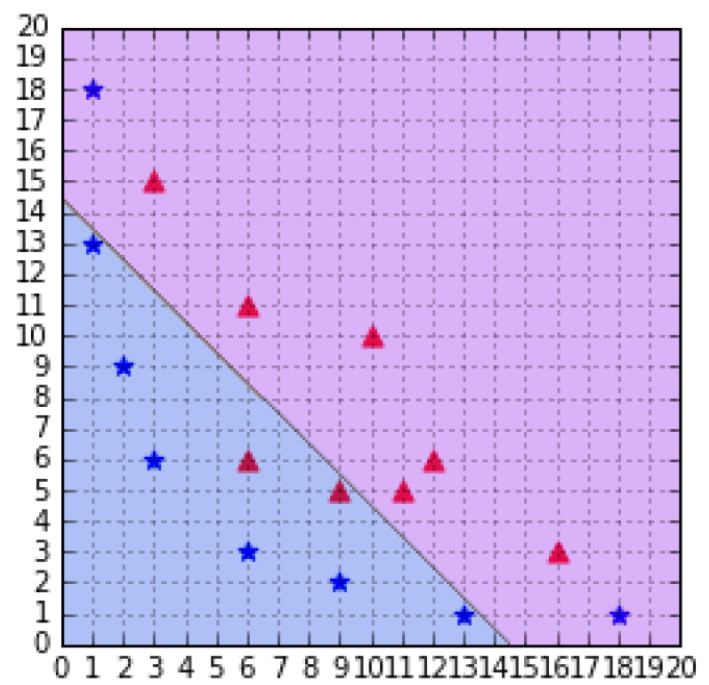
\includegraphics[width=1\textwidth]{assets/svm/kernel__1.png}
      \subcaption*{$d=1$}
    \end{subfigure}\vspace*{1mm}
    \begin{subfigure}{0.2\textwidth}
      \centering
      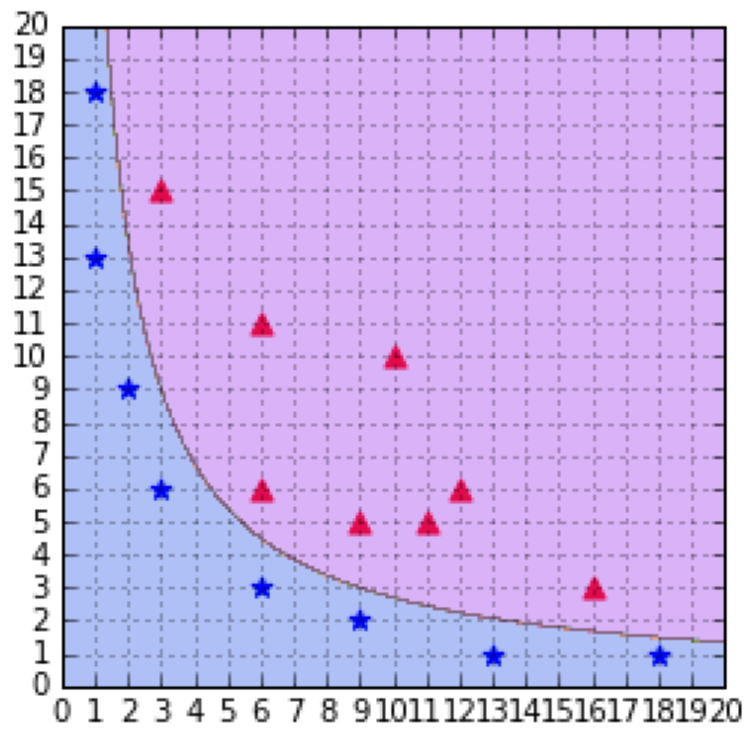
\includegraphics[width=1\textwidth]{assets/svm/kernel__2.png}  
      \subcaption*{$d=2$}     
    \end{subfigure}\vspace*{1mm}
    \begin{subfigure}{0.21\textwidth}
      \centering
      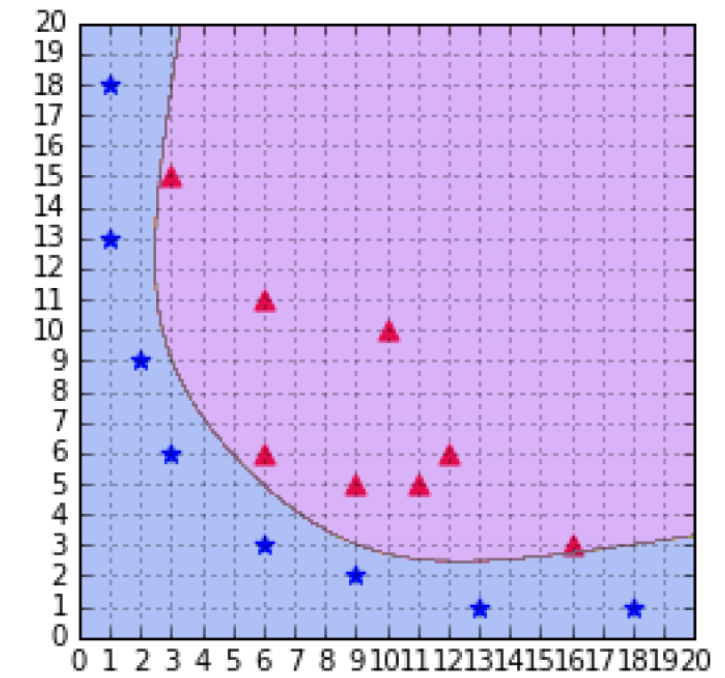
\includegraphics[width=1\textwidth]{assets/svm/kernel__6.png}  
      \subcaption*{$d=6$}     
    \end{subfigure}
  \end{figure*}
  \item Alternatively, there are e.g. \textbf{circular kernels}, since some data can't be separated by any polynomial.
  \begin{figure*}[ht]
    \centering
    \begin{subfigure}{0.2\textwidth}
      \centering
      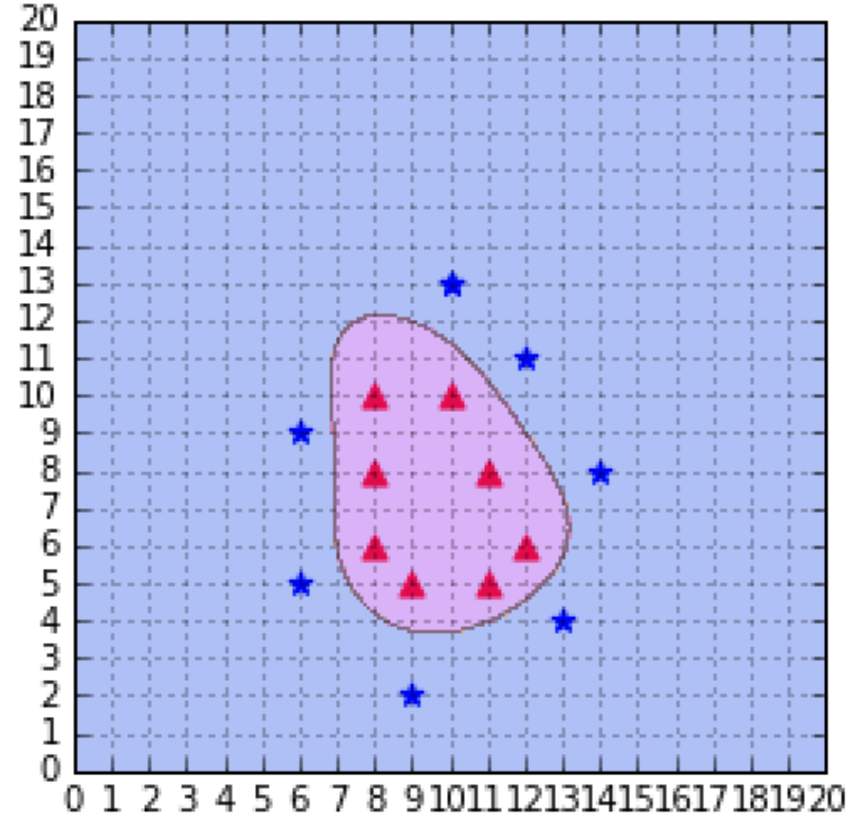
\includegraphics[width=1\textwidth]{assets/svm/kernel__circular.png}
    \end{subfigure}
  \end{figure*}
\end{itemize}

